\chapter{Cross-Lingual Word Sense Disambiguation}
\label{chap:clwsd}



In this chapter we apply k-nearest neighbour classifiers to two similar and
localised translation tasks organized for SemEval 2010: Cross-Lingual Word
Sense Disambiguation and Cross-Lingual Lexical Substitution.  Both tasks aim to
disambiguate a marked word in context by finding an appropriate translation for
it in another language. Our system, UvT-WSD1 participates for the two tasks and
achieves winning scores for the former. With a later rewrite of our system,
called WSD2, we focus on hyperparameter optimisation and participate again in
the Cross-Lingual Word-Sense Disambiguation task for SemEval 2013. We then
achieve winning scores for four of the five language pairs, when asked to
predict the best translation(s). Our final results, however, indicate that
hyperparameter optimisation did not lead to the best results, indicating
overfitting by our optimisation method in this aspect. Feature selection does
have a modest positive impact.


\nobibliography*
\textsc{This chapter is based on the following two publications: }
\begin{NoHyper}\bibentry{WSD1}
\bibentry{WSD2}\end{NoHyper}




\section{Introduction}

The UvT-WSD1 system we introduce here took part in two similar SemEval 2010
tasks: Cross-Lingual Word Sense Disambiguation \citep{WSD} and Cross-Lingual
Lexical Substitution \citep{CLLS}. In each task, a number of polysemous words is
selected for which the senses are to be determined for a number of instances of
these words. For each word, a number of samples in context is provided, where
each sample consists of one sentence, with the word to be disambiguated marked.

%This approach suggests that Word Sense Disambiguation and Machine Translation
%are related disciplines.
Because of the cross-lingual nature of the tasks, a word sense corresponds to a
translation in another language, rather than a sense description in the same
language. In the Cross-lingual Lexical Substitution task, the target language
is Spanish. The task is to find Spanish substitutes for the English words
marked in the test samples. In the Cross-Lingual Word Sense Disambiguation
task, we participate for English-Dutch and English-Spanish. The Word Sense
Disambiguation task provides training data for all five languages, in the form
of the sentence-aligned Europarl parallel corpus \citep{EUROPARL}. This is the
source of training data our UvT-WSD1 system uses for both tasks.

The system may output several senses per instance, rather than producing just
one sense prediction. These are evaluated in two different ways. The scoring
type ``\textbf{best}'' expects that the system outputs the best senses, in the
order of its confidence. The scoring type ``\textbf{out of five/ten}'' expects
five or ten guesses, and each answer weighs the same. These metrics are more
extensively described in \citep{CLLS}. The UvT-WSD1 system participates in both
scoring types, for both tasks. The system put forth in this paper follows a
similar approach as described in earlier research by \citep{Hoste+02}.

WSD2 is a rewrite and extension of our UvT-WSD1. In WSD2 we introduce and test
a new level of hyperparameter optimisation. We now participate for all five
target languages (Dutch, Spanish, Italian, French, and German). The task
presents twenty polysemous nouns with fifty instances each to be mapped onto
normalised (lemmatised) translations in all languages. The task is described in
detail in \citep{CLWSD2013TASKPAPER}.

Trial data is provided and has been used to optimise system
parameters. Due to the unsupervised nature of the task, no training data is
provided. However, given that the gold standard of the task is based
exclusively on the Europarl parallel corpus \citep{EUROPARL}, we select that
same corpus to minimise our chances of delivering translations that the human
annotators preparing the test data could have never picked.

\section{System Description}

Our system uses machine learning techniques to learn what
senses/translations are associated with any of the target words. It does so on
the basis of a variety of local and global context features, discussed in
Section \ref{sec:features}. At the core of the system are the classifiers, or
so called ``word experts'', one per target word. These are built using the
Tilburg Memory Based Learner (TiMBL) \citep{TIMBL}, making use of the IB1
algorithm, an implementation of the $k$-nearest neighbour classifier.

The core of the system can be subdivided into three stages. In the
first stage, the word-aligned parallel corpus is read and for each found
instance of one of the target words, features are extracted to be used in the
classifier. The class consists of the word aligned to the found instance of the
target word, i.e. the translation/sense. In this way a word expert is built for
each of the target words in the task, yielding a total amount of classifiers
equal to the total amount of target words. The test data is processed in a
similar way, for each marked occurrence of any of the target words, features
are extracted and test instances are created. Subsequently, the word experts
are trained and tested, and on the basis of the training data, a parameter
search algorithm \citep{PARAMSEARCH} determines the optimal set of classifier
parameters for each word expert, including for example the value of $k$ and the
distance weighting metric used.

In the last stage, the classifier output of each word expert is parsed. The
classifiers yield a distribution of classes per test instance, and these are
converted to the appropriate formats for ``best'' and ``out of five/ten''
evaluation. For the latter scoring type, the five/ten highest scoring senses
are selected, for the former scoring type, all classes scoring above a certain
threshold are considered ``best''. The threshold is set at $90\%$ of the score
of the highest scoring class.

\subsection{Word-Alignment, Tokenisation, Lemmatisation and Part-of-Speech-tagging}

The Europarl parallel corpus, English-Spanish and English-Dutch, is delivered
as a sentence-aligned parallel corpus. We subsequently run GIZA++ \citep{GIZA}
to compute a word-aligned parallel corpus.

This, however, is not the sole input. The target words in both tasks are
actually specified as a lemma and part-of-speech tag pair, rather than words.
In the Word Sense Disambiguation task, all target lemmas are simply nouns, but
in the Cross-Lingual Lexical Substitution task, they can also be verbs,
adjectives or adverbs. Likewise, both tasks expect the sense/translation output
to also be in the form of lemmas. Therefore the system internally has to be
aware of the lemma and part-of-speech tag of each word in the parallel corpus
and test data, only then can it successfully find all occurrences of the target
words. In order to get this information, both sides of the word-aligned
parallel corpus are run through tokenisers, lemmatisers and Part-of-Speech
taggers, and the tokenised output is realigned with the untokenised input so
the word alignments are retained. The test data is also processed this way. For
English and Spanish, the software suite Freeling \citep{FREELING} performed all
these tasks, and for Dutch it was done by Tadpole \citep{TADPOLE}, a previous
version of what is currently called Frog.

\subsection{Feature Extraction}
\label{sec:features}

The system can extract a variety of features to be used in training and
testing. A distinction can be made between \emph{local context features} and
\emph{global context features}. Local context features are extracted from the
immediate neighbours of the occurrence of the target word. One or more of the
following local context features are extractable by the UvT-WSD1 system: word
features, lemma features, and part-of-speech tag features. In each case, $n$
features both to the right and left of the focus word are selected. Moreover,
the system also supports the extraction of bigram features, but these did not
perform well in the experiments.

The global context features are made up of a bag-of-words representation of
keywords that \emph{may} be indicative for a given word to sense/translation
mapping. The idea is that words are collected which have a certain power of
discrimination for the specific target word with a specific sense, and all such
words are then put in a bag-of-word representation, yielding as many features
as the amount of keywords found. A global count over the full corpus is needed
to find these keywords. Each keyword acts as a binary feature, indicating
whether or not that particular keyword is found in the context of the
occurrence of the target word. The context in which these keywords are searched
for is exactly one sentence, i.e. the sentence in which the target word occurs.
This is due to the test data simply not supplying a wider context.

The method used to extract these keywords ($k$) is proposed by \citep{NgL96} and
used also in the research of \citep{Hoste+02}. Assume we have a focus word $f$,
more precisely, a lemma and part-of-speech tag pair of one of the target words.
We also have one of its aligned translations/senses $s$, which in this
implementation is also a lemma. We can now estimate $P(s|k)$, the probability
of sense $s$, given a keyword $k$, by dividing $N_{s,k_{local}.}$ (the number
of occurrences of a possible local context word $k$ with particular focus word
lemma-PoS combination and with a particular sense $s$) by $N_{k_{local}}$ (the
number of occurrences of a possible local context keyword $k_{loc}$ with a
particular focus word-PoS combination regardless of its sense). If we also take
into account the frequency of a possible keyword $k$ in the complete training
corpus ($N_{k_{corpus}}$), we get:


\begin{equation}
P(s|k) = \frac{N_{s,k_{local}}}{N_{k_{local}}}(\frac{1}{N_{k_{corpus}}})
\end{equation}

\citep{Hoste+02} select a keyword $k$ for inclusion in the bag-of-words
representation if that keyword occurs more than $T_1$ times in that sense $s$,
and if $P(s|k) \ge T_2$. Both $T_1$ and $T_2$ are predefined thresholds, which
by default were set to $3$ and $0.001$ respectively. In addition, UvT-WSD1
contains an extra parameter which can be enabled to automatically adjust the
$T_1$ threshold when it yields too many or too few keywords. The selection of
bag-of-word features is computed prior to the extraction of the training
instances, as this information is a prerequisite for the successful generation
of both training and test instances.

\section{UvT-WSD1}
\label{sec:wsd1}

\subsection{Voting system}

The local and global context features, and the various parameters that can be
configured for extraction, yield a lot of possible classifier combinations.
Rather than merging all local context and global context features together in a
single classifier, they can also be split over several classifiers and have an
arbiter voting system do the final classification step. UvT-WSD1 also supports
this approach. A voter is constructed by taking as features the class output of
up to three different classifiers, trained and tested on the training data, and
mapping these features onto the actual correct sense in the training data. For
testing, the same approach is taken: up to three classifiers run on the test
data; their output is taken as feature vector, and the voting system predicts a
sense. This approach may be useful in boosting results and smoothing out
errors. In our experiments we see that a voter combination often performs
better than taking all features together in one single classifier. Finally,
also in the voter system there is a stage of automatic parameter optimisation
for TiMBL.

\subsection{Experiments and Results}

Both SemEval 2010 tasks have provided trial data upon which the system could be
tested during the development stage. Considering the high configurability of
the various parameters for feature extraction, the search space in possible
configurations and classifier parameters is vast, also due to fact that the
TiMBL classifier used may take a wealth of possible parameters. As already
mentioned, for the latter an automatic algorithm of parameter optimisation was
used \citep{PARAMSEARCH}, but optimisation of the feature extraction parameters
has not been automated. Rather, a selection of configurations has been manually
chosen and tested during the development stage

%TODO: explain metrics

% NOT IN ORIGINAL PAPER (likely due to space constraints)

In Table~\ref{tab:task3trialnl} some of the results on the \emph{trial data}
are listed, for the Dutch Word Sense Disambiguation task only.  All scores are
\emph{averaged} over the five target words in the trial data. Included is also
a baseline that has been computed by selecting simply the most common
translation/sense for each target word, regardless of the context it appears
in.

\begin{table}
\label{tab:task3trialnl}
\footnotesize{
\noindent\makebox[\textwidth][c]{%
\begin{tabular}{ll}
\hline
\textbf{Feature configuration} & \textbf{Accuracy} \\%& \textbf{Mode PR} \\
\hline
Voter: word2$+$lemma2 \& global & \textbf{14.45} \\%& 19.21 \\
word2$+$lemma2 & 14.09 \\%& 19.21 \\
word2 & 13.30 \\%& 20.07 \\
word2$+$global & 13.09 \\%& 22.96 \\
global & 12.78 \\%& 17.19 \\
word3 & 12.68 \\%& 18.52 \\
word1 & 12.61 \\%& 14.08 \\
word2$+$pos2$+$lemma2 & 11.03 \\%& 12.21 \\
baseline & 10.82 \\% & 22.36 \\
\hline
\end{tabular}}
\caption{Average scores for various configurations on the trial data of the English-\emph{Dutch} Word Sense Disambiguation
    task, averaged over five target words. At the time this experiment was conducted, a bug existed in the output format specification, resulting in slightly lower scores.}
}
\end{table}

In Table~\ref{tab:task3trialnl},``word'' refers to the surface forms of the
words, ``lemma'' denotes lemma features, ``pos'' denotes Part-of-Speech
information. The subsequent number refers to the local context size. The
``global'' configuration refers to global context features.

%/NOT IN ORIGINAL PAPER

The following two configurations of features were assembled for submission to
the final shared task:

\begin{enumerate}
\item \textbf{UvT-WSD1-v} (aka \emph{UvT-v}) -- An arbiter-voting system over
three classifiers: 1) Word experts with two word features and lemma features on
both sides of the focus word. 2) Word experts with global features\footnote{For
the Cross-Lingual Lexical Substitution task only, the parameter to recompute
the $T_1$ threshold automatically was enabled.}. 3) Word experts with two word
features, two lemma features \emph{and} two part-of-speech tag features.
\item \textbf{UvT-WSD1-g} (aka \emph{UvT-g}) -- Word experts with global features
only.
\end{enumerate}

The UvT-v configuration was selected for its best performance of the trial
chance\footnote{An extra configuration with PoS information was included in the
voter on the odd chance it can make a difference, despite the poor performance
observed in Table~\ref{tab:task3trialnl}}. The UvT-g configuration was included
to judge the efficacy of global context features when used standalone.

Table~\ref{tab:uvtwsd1clls} shows a condensed view of the results for the Cross-Lingual Lexical
Substitution task. Table~\ref{tab:uvtwsd1clwsd} shows the final results for the Word-Sense
Disambiguation task. Note that UvT-WSD1-v and UvT-WSD1-g are two different
configurations of the UvT-WSD1 system, and to conserve space these are
abbreviated as UvT-v and UvT-g respectively. These are also the names used in
both tasks \citep{WSD,CLLS} to refer to our system.

\begin{table}
%\begin{tabular}{|l|c|c||l|c|c|}
\footnotesize{
\noindent\makebox[\textwidth][c]{%
\begin{tabular}{lcc}
\hline
%\textbf{BEST} & UvT-v & UvT-g & \textbf{OUT OF TEN} & UvT-v & UvT-g \\
%Precision \& Recall & 21.09 & 43.76 & & 58.91 & 55.29 \\
%Mode Prec. \& Rec. & 19.59 & 41.02 & &  62.96 & 73.94 \\
%Ranking (out of 14) & 6 & 9 & & 3 & 4 \\
\textbf{BEST} & UvT-WSD1-v & UvT-WSD1-g \\
Precision \& Recall & 21.09 & 19.59 \\
Mode Prec. \& Rec. & 43.76 & 41.02  \\
Ranking (out of 14) & 6 & 9 \\
\hline
\textbf{OUT OF TEN} & UvT-WSD1-v & UvT-WSD1-g \\
Precision \& Recall &  58.91 & 55.29 \\
Mode Prec. \& Rec. &  62.96 & 73.94 \\
Ranking & 3 & 4 \\
\hline
\end{tabular}}
\caption{UvT-WSD1 results in the Cross-Lingual Lexical Substitution task}
\label{tab:uvtwsd1clls}
}
\end{table}

\begin{table*}
\footnotesize{
\noindent\makebox[\textwidth][c]{%
\begin{tabular}{lccccc}
\hline
\textbf{Dutch BEST} & UvT-v & UvT-g & T3-COLEUR & &  \\
Precision \& Recall & 17.7 & 15.93 & 10.72 \& 10.56  & & \\
Mode Prec. \& Rec. & 12.06 & 10.54 & 6.18 \& 6.16 & & \\
\hline
\textbf{Dutch OUT OF FIVE} & UvT-v & UvT-g & T3-COLEUR
 & & \\
Precision \& Recall & 34.95 & 34.92 & 21.54 \& 21.22 & & \\
Mode Prec. \& Rec. & 24.62 & 19.72 & 12.05 \& 12.03 & & \\
\hline
\textbf{Spanish BEST} & UvT-v        & UHD-1 & UvT-g & T3-COLEUR & FCC-WSD1 \\
Precision \& Recall & 23.42 & 20.48 \& 16.33 &  19.92 & 19.78 \& 19.59 & 15.09\\
Mode Prec. \& Rec. & 24.98 & 28.48 \& 22.19 & 24.17 & 24.59 & 14.31 \\
\hline
\textbf{Spanish OUT OF FIVE} & UvT-g & UvT-v & FCC-WSD2 & UHD-1 & T3-COLEUR \\
Precision \& Recall  & 43.12 & 42.17 & 40.76 & 38.78 \& 31.81 & 35.84 \& 35.46 \\
Mode Prec. \& Rec. & 43.94 & 40.62 & 44.84 & 40.68 \& 32.38 & 39.01 \& 38.78 \\
\hline
\end{tabular}}
\caption{UvT-WSD1 results in comparison to other participants in the Word-Sense Disambiguation task. Only whenever two values are given, precision and recall are not equal. }
\label{tab:uvtwsd1clwsd}
}
\end{table*}

\section{WSD2}
\label{sec:wsd2}

\subsection{Feature and Hyperparameter Optimisation}

The size of the local context, the inclusion of global context features, and
the inclusion of syntactic features are all features that can be selected,
changed, or disabled, allowing for a variety of combinations to be tested. In
addition, each word expert is a $k$-nearest neighbour classifier that can take
on many hyperparameters beyond $k$. For our participation in the SemEval 2013
Cross-Lingual Word Sense Disambiguation task, with our WSD2 system, we performed both
optimisations for all word experts. The optimisations, however, were performed
independently to reduce complexity: we optimised classifier hyperparameters on
the basis of the training examples extracted from our parallel corpus,
producing optimal accuracy on each word-expert. We optimised feature selection
on the basis of the trial data provided for the task. As has been argued before
\citep{Hoste+02}, the joint search space of feature selection and
hyperparameters is prohibitively large. Our current setup runs the risk of
finding hyperparameters that are not optimal for the feature selection in the
second optimisation step. Our final results indeed show that only feature
selection produced improved results. We choose the feature selection with the
highest score on the trial set, for each of the nouns and separately for both
evaluation metrics in the task.

To optimise the choice of hyperparameters per word expert, a heuristic
parameter search algorithm
\citep{PARAMSEARCH}\footnote{https://github.com/LanguageMachines/paramsearch} was used that
implements wrapped progressive sampling using cross-validation: it performs a
large number of experiments with many hyperparameter setting combinations on
small samples of training data, and then progressively zooms in on combinations
estimated to perform well with larger samples of the training data. As a
control run we also trained word experts with default hyperparameters, i.e.
with $k=1$ and with all other hyperparameters at their default values as
specified in the TiMBL implementation.

\subsection{Experiments \& Results}

To assess the accuracy of a certain configuration of our system as a whole, we
take the average over all word experts. An initial experiment on the trial data
explores the impact of different context sizes, with hyperparameter
optimisation on the classifiers. The results, shown in Figure~\ref{figcontext},
clearly indicate that on average the classifiers perform best with a local
context of just one word to the left and one to the right of the word to be
disambiguated. Larger context sizes have a negative impact on average accuracy.
These tests include hyperparameter optimisation, but the same trend shows
without.

%added for thesis:
It is interesting to put this in contrast with the results from UvT-WSD1 in
Table~\ref{tab:task3trialnl}, where a context size of two leads to better
results than context size one.  This can only be explained by the
difference in trial data. %TODO: what is the difference in trial data?
%/

\begin{figure}[t]
\noindent\makebox[\textwidth][c]{%
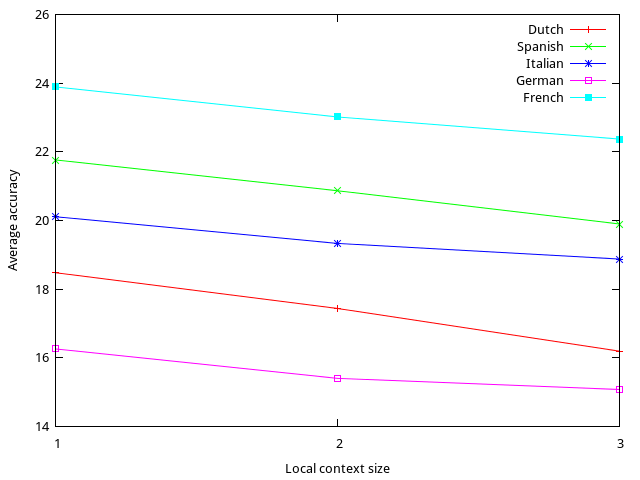
\includegraphics[width=8cm]{context.png}
}
\caption{Average accuracy for different local context sizes}
\label{figcontext}
\end{figure}

We submitted three configurations of our system to the shared task, the maximum
number of runs. Adding lemma features to the local context window of three
words, i.e. left word, focus word and right word, proves beneficial in general.
This is shown in Table~\ref{tab:trialresults}.  This is therefore the first
configuration we submitted (\texttt{c1l}). As second configuration
(\texttt{c1lN}) we submitted the same configuration without parameter
optimisation on the classifiers. Note that neither of these include global
context features.

\begin{table}[t]
\footnotesize
\noindent\makebox[\textwidth][c]{%
\begin{tabular}{lrrrrr}
\hline
\textbf{BEST} & \textbf{ES} & \textbf{FR} & \textbf{IT} & \textbf{NL} & \textbf{DE} \\
\hline
baseline &  19.65 & 21.23 & 15.17 & 15.75 & 13.16 \\
plain & 21.76 & 23.89 & 20.10 & 18.47 & 16.25 \\
$+$lem (\texttt{c1l}) & 21.88 & \textbf{23.93} & \textbf{19.90} & \textbf{18.61} & \textbf{16.43} \\
$+$pos & 22.09 & 23.91 & 19.95 & 18.02 & 15.37 \\
lem$+$pos & \textbf{22.12} & 23.61 & 19.82 & 18.18 & 15.48 \\
glob.context & 20.57 & 23.34 & 17.76 & 17.06 & 16.05 \\
\hline
\textbf{OUT-OF-5} & \textbf{ES} & \textbf{FR} & \textbf{IT} & \textbf{NL} & \textbf{DE} \\
\hline
baseline & 48.34 & 45.99 & 34.51 & 38.59 & 32.90 \\
plain & 49.81 & \textbf{50.91} & 42.30 & 41.74 & \textbf{36.86} \\
$+$lem (\texttt{c1l}) & \textbf{49.91} & 50.65 & \textbf{42.41} & \textbf{41.83} & 36.45 \\
$+$pos & 47.86 & 49.72 & 41.91 & 41.31 & 35.93 \\
lem$+$pos & 47.90 & 49.75 & 41.49 & 41.31 & 35.80 \\
glob.context & 48.09 & 49.68 & 40.87 & 37.70 & 34.47 \\
\hline
\end{tabular}}
\caption{Feature exploration on the trial data}
\label{tab:trialresults}
\end{table}

The third configuration (\texttt{var}) we submitted includes feature selection,
and selects per word expert the configuration that has the highest score on the
trial data, and thus tests all kinds of configurations. Note that
hyperparameter optimisation is also enabled for this configuration. Due to the
feature selection on the trial data, we by definition obtain the highest scores
on this trial data, but this carries the risk of overfitting. Results on the
trial data are shown in Table~\ref{tabpar}.

\begin{table}
\footnotesize
\noindent\makebox[\textwidth][c]{%
\begin{tabular}{lrrrrr}
\hline
\textbf{BEST} & \textbf{ES} & \textbf{FR} & \textbf{IT} & \textbf{NL} & \textbf{DE} \\
\hline
c1lN & 22.60  & 24.09 & 19.87 & 18.70 & 16.43 \\
c1l & 21.88 & 23.93 & 19.90 & 18.61 & 16.43 \\
var & 23.79 & \textbf{25.66} & \textbf{21.65} & \textbf{20.19} & \textbf{19.06} \\
varN & \textbf{23.90} &  25.65 & 21.52 & 19.92 & 18.96 \\
\hline
\textbf{OUT-OF-5} &  \textbf{ES} & \textbf{FR} & \textbf{IT} & \textbf{NL} & \textbf{DE} \\
\hline
c1lN & 50.14 & 50.98 & 42.92 & 42.08 &  36.45 \\
c1l & 49.91 & 50.65 & 42.41 & 41.83 & 36.45 \\
var & 51.95 & \textbf{53.66} & 45.59 & \textbf{44.66} & \textbf{39.81} \\
varN & \textbf{52.91} & 53.61 & \textbf{45.92} & 44.32 & 39.40 \\
\hline
\end{tabular}}
\caption{Results on the trial data}
\label{tabpar}
\end{table}

The hyperparameter optimisation on classifier accuracy has a slightly negative
impact, suggesting overfitting on the training data. Therefore a fourth
configuration (\texttt{varN}) was tried later to independently assess the idea
of feature selection, without hyperparameter optimisation on the classifiers.
This proves to be a good idea. However, the fourth configuration was not yet
available for the actual competition. This incidentally would have had no
impact on the final ranking between competitors. When we run these systems on
the actual test data of the shared task, we obtain the results in
Table~\ref{tabfinal}. The best score amongst the other competitors is mentioned
in the last row for reference, this is the HLTDI team \citep{HLTDI} for all but
Best-Spanish, which goes to the NRC contribution \citep{CARPUAT}.

\begin{table}[tbh]
\footnotesize
\noindent\makebox[\textwidth][c]{%
\begin{tabular}{lrrrrr}
\hline
\textbf{BEST} & \textbf{ES} & \textbf{FR} & \textbf{IT} & \textbf{NL} & \textbf{DE} \\
\hline
baseline & 23.23 & 25.74 & 20.21 & 20.66 & 17.42 \\
c1l &  28.40 & 29.88 & 25.43 & 23.14 & 20.70 \\
c1lN &  28.65 & 30.11 & \textbf{25.66} & \textbf{23.61} & 20.82 \\
var & 23.3 & 25.89 & 20.38 & 17.17 & 16.2 \\
varN & 29.05 & \textbf{30.15} & 24.90 & 23.57 & \textbf{21.98} \\
best competitor & \textbf{32.16} & 28.23 & 24.62 & 22.36 & 19.92 \\
\hline
\textbf{OUT-OF-5} & \textbf{ES} & \textbf{FR} & \textbf{IT} & \textbf{NL} & \textbf{DE} \\
\hline
baseline & 53.07 & 51.36 & 42.63 & 43.59 & 38.86 \\
c1l &  58.23 & 59.07 & 52.22 & \textbf{47.83} & 43.17 \\
c1lN & 57.62 & \textbf{59.80} & 52.73 & 47.62 & 43.24 \\
var & 55.70 & 59.19 & 51.18 & 46.85 & 41.46 \\
varN & 58.61 & 59.26 & 50.89 & 50.42 & 43.34 \\
best competitor & \textbf{61.69} & 58.20 & \textbf{53.57}  & 46.55 & \textbf{43.66} \\
\hline
\end{tabular}}
\caption{Results on the test set}
\label{tabfinal}
\end{table}

A major factor in this task is the accuracy of lemmatisation, and to lesser
extent of PoS tagging. We conducted additional experiments on German and French
without lemmatisation, tested on the trial data. Results immediately fell below
baseline.

Another main factor is the quality of the word alignments, and the degree to
which the found word alignments correspond with the translations the human
annotators could choose from in preparing the gold standard. An idea we tested
is, instead of relying on the mere intersection of word alignments, to use a
phrase-translation table generated by and for the Statistical Machine
Translation system Moses \citep{Koehn+07}, which uses the grow-diag-final
heuristic to extract phrase pairs. This results in more phrases, and whilst
this is a good idea for MT, in the current task it has a detrimental effect, as
it creates too many translation options and we do not have an MT decoder to
discard ineffective options in this task. The grow-diag-final heuristic
incorporates unaligned words to the end of a translation in the translation
option, a bad idea for CLWSD.


\section{Discussion and Conclusion}

%Cross-Lingual Word Sense Disambiguation and Cross-Lingual Lexical Substitution
%have proven to be hard tasks, with scores that are relatively close to
%baseline.


%It has to be noted that the approach laid out here is built around word
%experts. Some word experts may perform well in a certain configuration, and
%others may perform worse. This is also a more general fact: some words seem
%notably harder than others, and perform worse in any configuration.

In our UvT-WSD1 system, we used the same configuration of feature extraction,
or a voter over a predetermined set of configurations, for all word experts. The actual
classifier parameters however, do differ per word expert, as they are the
result of the automatic parameter optimisation algorithm. Our WSD2 system
takes parameter optimisation one step further by selecting system parameters
per word expert from the best configurations on the trial data. Optimising the
hyperparameters of the classifiers on the training data proves to have a
slightly negative effect though, especially when combined with the selection of
features. This is likely due to the fact that feature selection was performed
after hyperparameter optimisation, causing certain optimisations to be rendered
ineffective.

Keeping in mind the fact that different word experts may perform differently,
some \emph{general} conclusions can be drawn from the experiments on the trial
data. It appears to be beneficial to include lemma features, rather than just
word features. Both the 2010 and 2013 tasks corroborate this. However, adding
Part-of-Speech features tends to have a negative impact. For these local
context features, the optimum context size is often two features to the left
and two features to the right of the focus word, cf.  \citep{Hendrickx+02}.

The global keyword features perform well for UvT-WSD1, but best results are
achieved if they are not mixed with the local context features in one
classifier. For WSD2 in the 2013 task, however, the global context features
make less an impact than even just the linguistically-uninformed local context
feature, as became clear from the the feature exploration stage in
Table~\ref{tab:trialresults}. As the keyword selection algorithm is the same
as in UvT-WSD1, this is surprising and must then be attributed to the dataset.
Taking into account the earlier discrepancy between the results of UvT-WSD1 and
WSD2, we may conclude that optimal configurations differ accross datasets.

For UvT-WSD1, an arbiter voting approach over multiple classifiers helps to smooth out errors
and yields the highest scores (see Tables \ref{tab:uvtwsd1clls} and
\ref{tab:uvtwsd1clwsd}). When compared to the other
participants, the UvT-WSD1 system in the voting configuration ranks first in
the Word Sense Disambiguation task, for the two language pairs in which we
participated. WSD2 does not use a voting approach, as it already explicitly
attempts to assess the efficacy of various hyperparameter optimisations and
feature selections.

When asked to predict the best translation(s), our WSD2 system comes out on top
for four out of five languages in the SemEval 2013 task; only for Spanish we
are surpassed by two competitors. Our out-of-five predictions win for two out
of five languages, and are fairly close the the best competitor for the others,
except again for Spanish. It is interesting to observe that, due to our feature
selection without hyperparameter optimisation on the classifier not being
available yet at the time of submission, our simplest system \texttt{c1lN}
emerged as best in the contest.

We assumed independence between hyperparameter optimisation and feature
selection, where the former was conducted using cross-validation on the
training data rather than on the development set. As this independence
assumption is a mere simplification to reduce algorithmic complexity, future
research could focus on a more integrated approach and test hyperparameter
optimisation of the classifiers on the trial set which may produce better
scores.

The WSD2 system is available as open-source under the GNU Public License v3. It
is implemented in Python \citep{PYTHON} and can be obtained from
http://github.com/proycon/wsd2\footnote{git commit
f10e796141003d8a2fbaf8c463588a6d7380c05e represents a fair state of the system
at the time of submission}. The experimental data and output of our
participation in the 2013 SemEval task are included in
this git repository as well.

